\documentclass{article}
\usepackage[letterpaper]{geometry}
\usepackage{graphicx}
\usepackage{xcolor}
\usepackage{amsmath}

% typesetting
% Margins and typesetting
\setlength{\textwidth}{5.00in}
\setlength{\oddsidemargin}{3.25in}
\addtolength{\oddsidemargin}{-0.5\textwidth}
\addtolength{\topmargin}{-0.55in}
\addtolength{\textheight}{2.00in}
\linespread{1.08}
\pagestyle{myheadings}
\markboth{}{\color{gray}\sffamily Hogg \& Villar / \texttt{MNIST-plus-plus}}
\sloppy\sloppypar\raggedbottom\frenchspacing
\renewcommand{\paragraph}[1]{\par\medskip\noindent\textbf{#1} ---}
\newcommand{\figref}[1]{\figurename~\ref{#1}}

\title{\bfseries \texttt{MNIST-plus-plus}: Toy datasets and challenges for equivariant machine learning and reasoning} 
\author{David W. Hogg,  Soledad Villar, others}
\date{}

\begin{document}

\maketitle\thispagestyle{empty}

\begin{abstract}\noindent
    The recognition and reading of text, and recognition of objects, often happens in the context of non-trivial perspective, object orientation, and geometry variations.
    The objective of this paper is to introduce toy problems for classification and reasoning with geometry and geometric symmetries in play.
    We provide four datasets and seven challenges based on simple transformations of the MNIST and Fashion-MNIST datasets.
    Some of the learning tasks are to recognize objects and handwritten digits in images that have had geometric transformations applied; some are to identify the geometric transformations themselves.
    The images are designed to contain enough context to determine (in most cases) both the image contents and the geometric transformations.
    We train standard-issue CNNs to deliver baseline performances on the learning tasks.
    [SOME SUMMARY OF CNN RESULTS HERE]
    One of the tasks---\texttt{MNIST+4}---involves identifying ordered sets of numbers in a transformed image; it is a true reasoning task and is therefore expected to be challenging for contemporary machine-learning methods.
\end{abstract}

\section{Introduction}

Real-world tasks require us to identify objects in arbitrary orientations and also make inferences about the orientations themselves, using context. 
See Figure~\ref{fig:example} for example images containing many objects in different orientations.
These images inspire recognition tasks that are interesting from a learning perspective, but also have industrial and commercial uses.
The objective of this contribution is to provide toy datasets that represent baby steps towards general recognition and geometric inference tasks.
These datasets directly generate challenges for learning and reasoning methods.

Individual letters, numbers, and symbols can only be reliably read in certain orientations.
For examples, Ws and Ms, 6s and 9s, ps and ds, 8s and $\infty$s, and so on, cannot be distinguished easily without some understanding of the orientation in which they were written, or intended to be read.
Despite this, when capable human readers pick up pieces of paper with writing or printing on it, they have no trouble orienting them correctly.
How does a human reliably orient a paper for reading?
The human finds the orientation that makes the majority of the characters easy to read, in which the writing makes sense or can be used for subsequent tasks.
What would happen if a paper contained only 6s or only Ws?
In this case the paper would not say much of interest!
But it also would be impossible to confidently orient.
So (somehow) it is the diversity of the characters on the page that sets the page orientation.

Individual handwritten digits are the content of what might be the most important standardized dataset in all of machine learning---the MNIST dataset \cite{mnist}.
As of writing, this dataset has more than 10,000 citations and many spin-off projects such as spherical-MNIST \cite{spherical}, and Fashion-MNIST \cite{fashion}.
The learning task for MNIST is very simple---identify the handwritten digit from 0 to 9---given oriented, black-and-white thumbnail images.
This task is explicitly \emph{not} an equivariant or geometric task.
All of the digits are given in standard Roman orientations.
Indeed, MNIST recognition projects coming from equivariant machine learning, which enforce invariances or equivariances with respect to rotations and reflections, have the property that they fail to distinguish 6s from 9s, among other pathologies \cite{something}.

In the Real World (tm), printed or captured visual information (letters, digits, images, and symbols) is not always (and maybe not even often) presented to us in an oriented way.
We must orient the print or image before reading it or interpreting it.
Therefore it is natural to consider an augmented version of MNIST, in which the digits have been arbitrarily reoriented.
However, that doesn't make a good reading task:
Individual decontextualized handwritten digits may not be identifiable after rotations or reflections (6s and 9s, 2s and 5s, or even 2s and 6s may look indistinguishable after these transformations).
In natural contexts, 6s and 9s are not read in isolation; they are read as part of a document or signage context where orientation can be inferred from surrounding characters and features.
Thus we can make data that is invariant to rotations, but which includes enough contextual information in each image to determine orientations and parities at reading or recognition time.

In what follows, we make four datasets and seven learning challenges, all of which are designed to be swap-in replacements for MNIST and Fashion-MNIST, and all of which are drawn from geometric distributions that are either exactly or approximately invariant to rotations and reflections.
The digit-reading tasks are designed to provide enough context to permit unambiguous reading of most data examples.
In addition to publishing these datasets, we have trained standard XXXX MODELS to provide unsophisticated baseline performance on all seven learning tasks.
Since these trained models incorporate no geometric symmetries, the baselines they provide should be easy to crush.

\section{Datasets and learning tasks}

\paragraph{Dataset 1: \texttt{Fashion++}}
The Fashion-plus-plus (\texttt{Fashion++}) dataset takes the Fashion-MNIST data \cite{fashion} and subjects it to random rotations and reflections.
The Fashion-MNIST dataset contains $28\times 28$ (CHECK) one-channel, 8-bit (\texttt{uint8}) black-and-white images of pieces of clothing from 10 discrete classes (labels).
These classes are 0--Top, 1--Trouser, 2--Pullover, 3--Dress, 4--Coat, 5--Sandal, 6--Shirt, 7--Sneaker, 8--Bag, and 9--Boot.

Each element of \texttt{Fashion++} is a randomly chosen element of Fashion-MNIST, subject to a randomly chosen linear transformation.
The transformation, in each case, is one of the 8 group elements of the dihedral group $D_4$ (CITE) generated by the 90-degree rotation and the reflection around the x-axis.
The dihedral group $D_4$ is the group of symmetries of the square.
Each element $M$ of the group can be represented as a $2\times 2$ matrix (given some coordinate ordering conventions).
In some sense, \texttt{Fashion++} is a pure data augmentation of Fashion-MNIST, except that the input Fashion-MNIST dataset and the output \texttt{Fashion++} dataset contain the same total numbers of images.
Because data elements were chosen randomly, some of the Fashion-MNIST input images are used more than once, and some are never used.
To prevent any spillage of information from training set to test set, we make the \texttt{Fashion++} training set only from the Fashion-MNIST training-set data, and we make the \texttt{Fashion++} test set only from the Fashion-MNIST test-set data. 

The \texttt{Fashion++} images are $28\times 28$ one-channel, 8-bit (\texttt{uint8}) black-and-white images.
Associated with each image is an integer label with one of ten values from 0 through 9 inclusive, representing the classes listed above.
In addition to the label, associated with each image is a 2x2 integer matrix $M$ which represents the group element that could be applied to rotate and reflect the image back to standard orientation.
There are eight different values for this 2x2 integer matrix.
There are 60,000 elements (image plus label plus group element) in the training set and 10,000 in the test set.
The first thirty-six elements of the \texttt{Fashion++} training set, along with their labels, are shown in \figref{fig:f}.
\begin{figure}[t!]
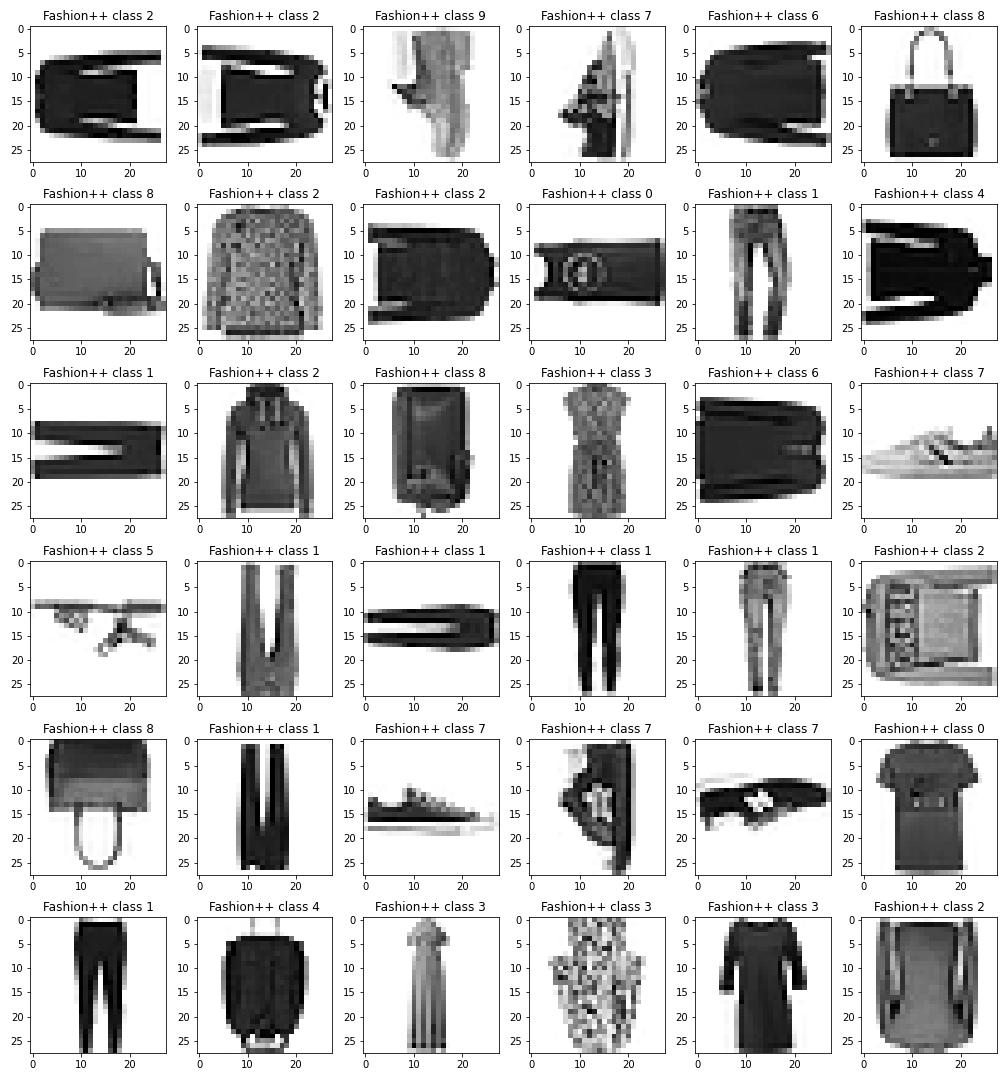
\includegraphics[width=\textwidth]{../notebooks/Fashion++.png}
\caption{The first 36 training-set images from the \texttt{Fashion++} dataset. The labels are given in the image titles.\label{fig:f}}
\end{figure}

\paragraph{Challenge 1: Infer \texttt{Fashion++} labels}
Identify the labels (classification).

\paragraph{Dataset 2: \texttt{MNIST+4}}

SOLE: Please put a citation to Bengio reasoning here. 
The benchmark dataset for reasoning tasks \cite{zhang2021pointer} is likely harder than ours. 

\begin{figure}[t!]
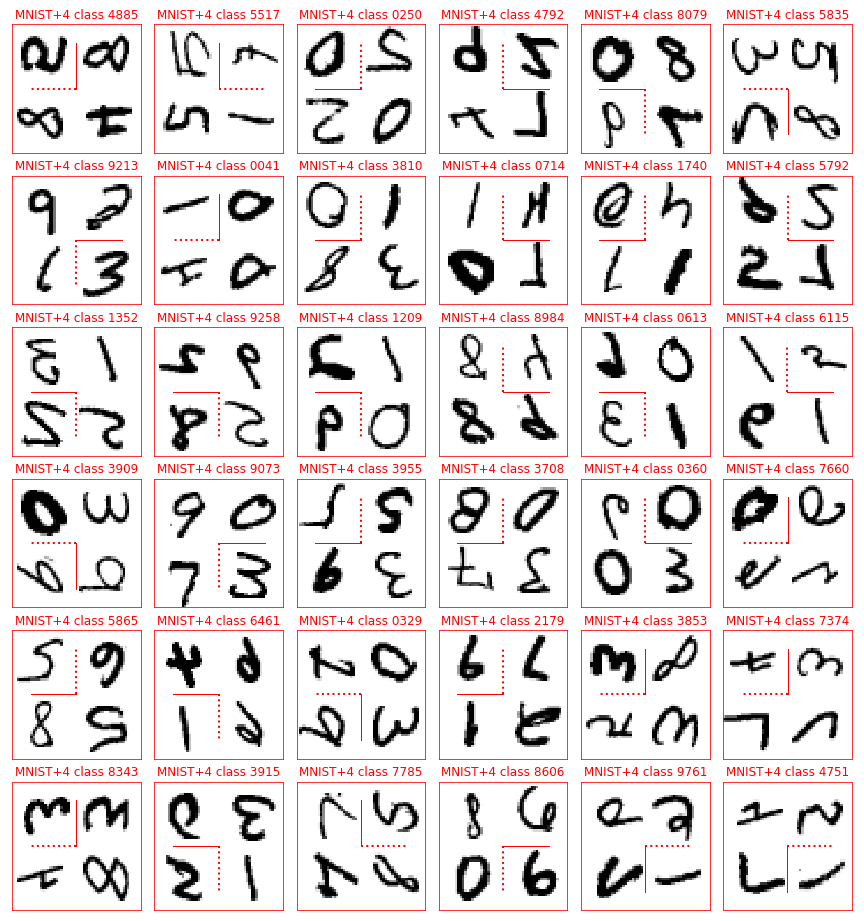
\includegraphics[width=\textwidth]{../notebooks/MNIST+4.png}
\caption{foo and bar.\label{fig:4}}
\end{figure}

\paragraph{Challenge 2: \texttt{MNIST+4} labels}
Identify the labels (classification and reasoning).
This has a reasoning component; note that some labels in the test set don't exist in the training set.
And yet humans can crush this (ish).

\paragraph{Challenge 3: \texttt{MNIST+4} group elements}
Foo and bar.

\paragraph{Dataset 3: \texttt{MNIST+9}}

\begin{figure}[t!]
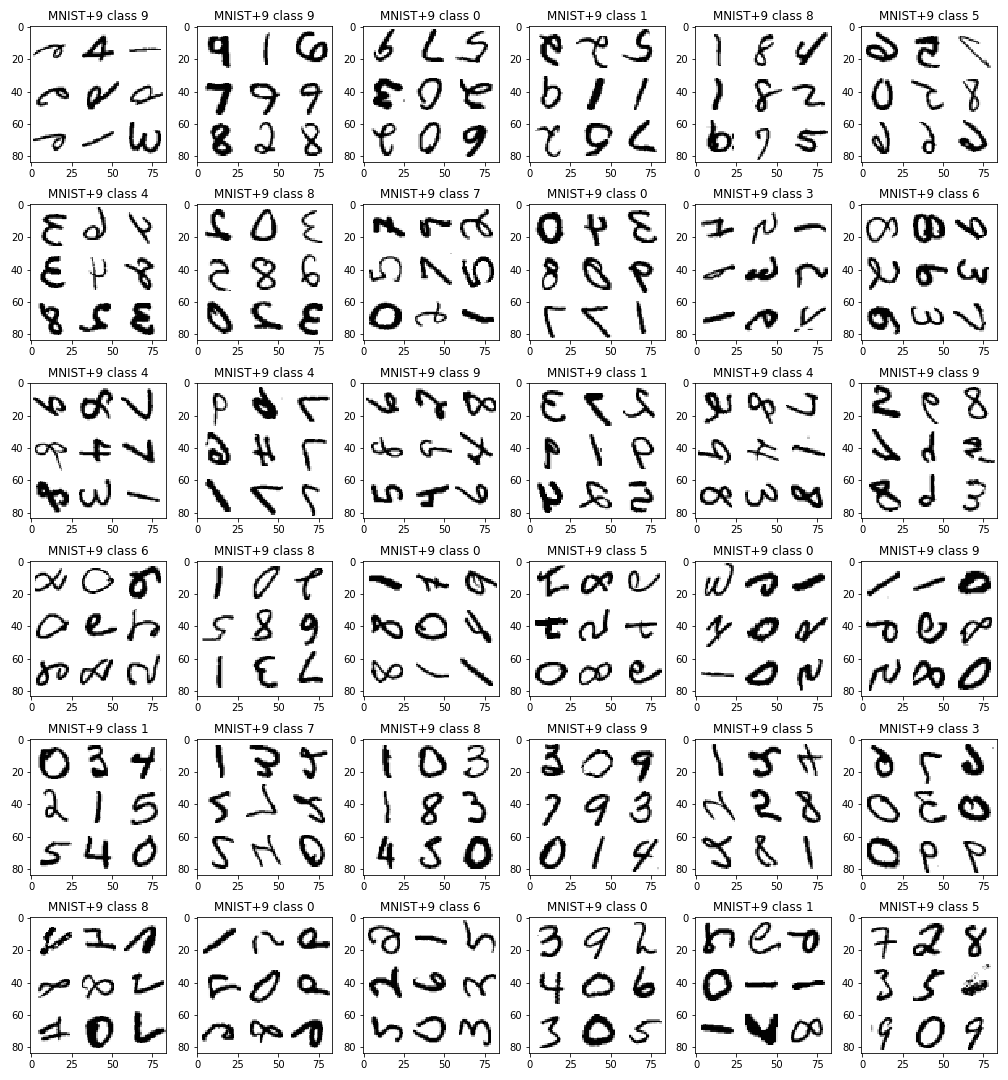
\includegraphics[width=\textwidth]{../notebooks/MNIST+9.png}
\caption{foo and bar.\label{fig:9}}
\end{figure}

\paragraph{Challenge 4: \texttt{MNIST+9} central digit labels}
Identify the labels (classification and reasoning).

\paragraph{Challenge 5: \texttt{MNIST+9} group elements}
Foo and bar.

\paragraph{Dataset 4: \texttt{MNIST+Inf}}

\begin{figure}[t!]
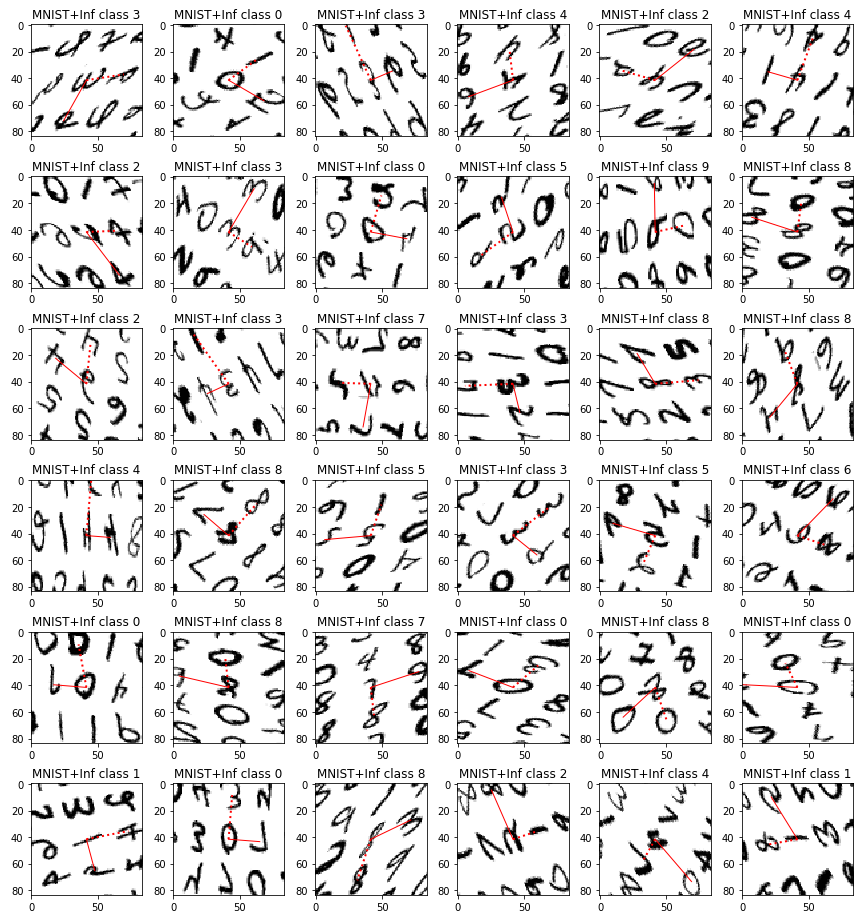
\includegraphics[width=\textwidth]{../notebooks/MNIST+Inf.png}
\caption{foo and bar.\label{fig:Inf}}
\end{figure}

\paragraph{Challenge 6: \texttt{MNIST+Inf} central digit labels}
Identify the labels (classification and reasoning).

\paragraph{Challenge 7: \texttt{MNIST+Inf} linear transformation operators}
Foo and bar. This is a regression!

\section{Baselines}

\section{Data download and discussion}

How do I get the data?

Comments about data augmentation.

Comments about reasoning?

\paragraph{Acknowledgements}
It is a pleasure to thank
  Wilson Gregory (JHU)
for valuable discussions.
SOLE GRANT NUMBERS.

\bibliographystyle{plain}
\raggedright
\bibliography{mnistplusplus}

\end{document}
